\begin{frame}{Giới hạn}
    \begin{tcolorbox}[colback=blue!10, colframe=blue!50!black, title=Định nghĩa]
    Giới hạn của hàm số \(f(x)\) tại điểm \(x=a\) được ký hiệu là:
    \begin{equation}
        \lim_{x \to a} f(x) = L
    \end{equation}
    là giá trị mà hàm số tiến tới khi \(x\) tiến tới \(a\).
    \end{tcolorbox}
\end{frame}
\newpage
\begin{frame}{Giới hạn}
    \begin{columns}
        \begin{column}{0.5\textwidth}
            Xét hàm số đồ thị hàm số \(y=x^2\) được phóng to gần điểm \((1; 1)\):
            \begin{figure}
            \centering
            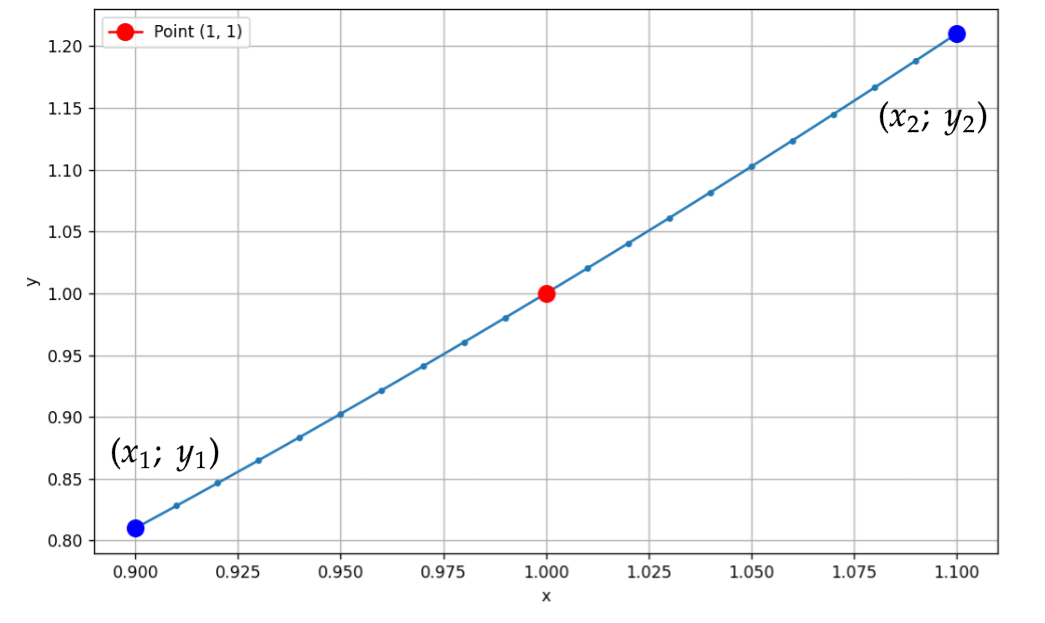
\includegraphics[width=1\textwidth]{Slides/figure/0.9-1.1.png}
            \end{figure}
        \end{column}
        \begin{column}{0.5\textwidth}
            \begin{itemize}
            \item \(y_1=x_1 ^2\) 
            \item \(y_2=x_2 ^2\)
            \end{itemize}
        \end{column}
    \end{columns}
\end{frame}
\newpage
\begin{frame}{Giới hạn}
    \begin{columns}
        \begin{column}{0.5\textwidth}
            Xét hàm số đồ thị hàm số \(y=x^2\) (bị gián đoạn) được phóng to gần điểm \((1; 1)\):
            \begin{figure}
            \centering
            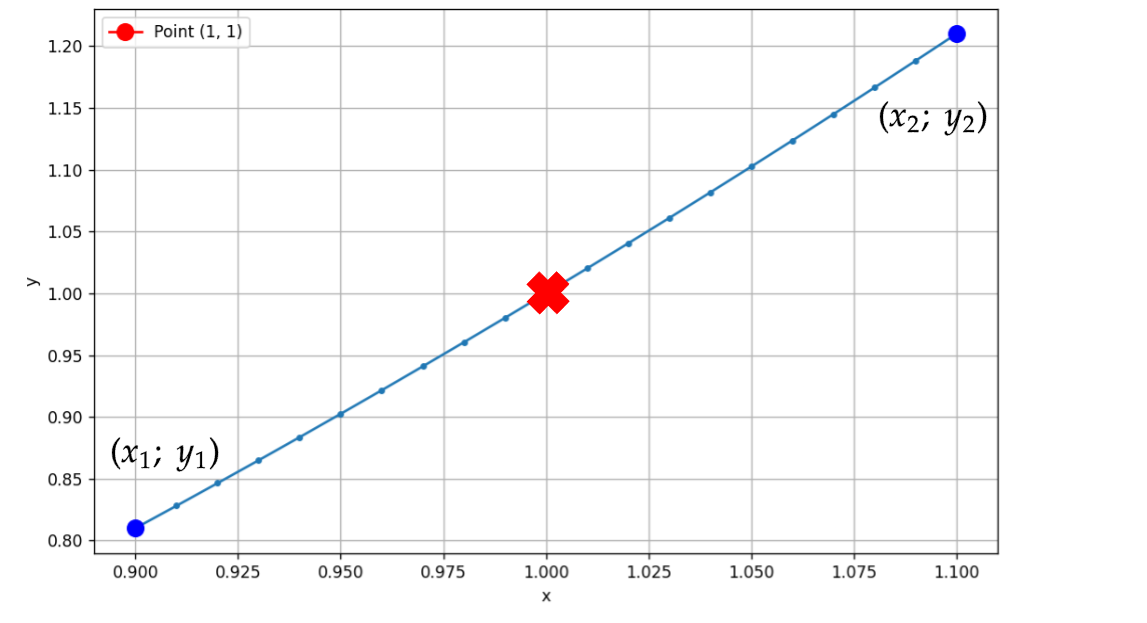
\includegraphics[width=1\textwidth]{Slides/figure/0.9-1.1 (drama).png}
            \end{figure}
        \end{column}
        \begin{column}{0.5\textwidth}
            \begin{itemize}
                \item \(y_1 = 
                \begin{cases}
                    x_1^2 & \text{nếu } x_1 \neq 1 \\
                    -100 & \text{nếu } x_1 = 1
                \end{cases}
            \)
            \item \(y_2 = 
                \begin{cases}
                    x_2^2 & \text{nếu } x_2 \neq 1 \\
                    100 & \text{nếu } x_2 = 1
                \end{cases}
            \)
            \end{itemize}
        \end{column}
    \end{columns}
\end{frame}
\newpage
\begin{frame}{Giới hạn}
    \begin{columns}
        \begin{column}{0.5\textwidth}
            \begin{table}[H]
        \centering
        \caption{Giá trị \( y = x^2 \) khi \( x \text{~tới gần } 1 \)}
        \begin{tabular}{|c|c||c|c|}
        \hline
        \multicolumn{2}{|c||}{Bên trái} & \multicolumn{2}{c|}{Bên phải} \\
        \hline
        \( x \) & \( y \) & \( x \) & \( y \) \\
        \hline
        0.900 & 0.8100 & 1.100 & 1.2100 \\
        0.925 & 0.8556 & 1.075 & 1.1556 \\
        0.950 & 0.9025 & 1.050 & 1.1025 \\
        0.975 & 0.9506 & 1.025 & 1.0506 \\
        0.990 & 0.9801 & 1.010 & 1.0201 \\
        0.995 & 0.9900 & 1.005 & 1.0100 \\
        0.999 & 0.9980 & 1.001 & 1.0020 \\
        \hline
        \end{tabular}
    \end{table}
        \end{column}
        \begin{column}{0.5\textwidth}
            \begin{itemize}
            \item \(y_1(1)=-100\)  
            \item \(y_2(1)=100\)
            \item \(\lim_{x_1 \to 1^{-}} y_1 = 1\)
            \item \(\lim_{x_2 \to 1^{+}} y_2 = 1\)
            \end{itemize}
        \end{column}
    \end{columns}
\end{frame}
